\chapter{Generelle statistiske begreber}
I dette appendiks defineres generelle statistiske begreber, som anvendes igennem rapporten.

Løst sagt, siges en estimator at være konsistent, hvis følgen $\boldsymbol{\theta}_n(\mathbf{Y})$ af estimatorer for parameteren $\boldsymbol{\theta}$ konvergerer i sandsynlighed mod den sande værdi $\boldsymbol{\theta}$. 
% 
\begin{defn}[Svag konsistens] \label{def:konsistent}
Lad $\{ \boldsymbol{\hat{\theta}}_n \}$ være en følge af estimatorer. Da siges $ \{ \boldsymbol {\hat{\theta}}_n \}$ at være konsistens for $\boldsymbol{\theta}$ hvis
\begin{align*}
\boldsymbol{\hat{\theta}} \overset{p}{\rightarrow} \boldsymbol{\theta}.
%\underset{n \rightarrow \infty}{\lim} P \left( \vert \boldsymbol{\hat{\theta}}_n - \boldsymbol{\theta} \vert \leq \epsilon \right) =1
\end{align*}
\end{defn}
%
\begin{defn}[Rod-n-konsistent estimator] \label{def:rodn}
En estimator $  \boldsymbol {\hat{\theta}}_n $ for $\boldsymbol{\theta}$ er rod-n-konsistent hvis
\begin{align*}
\boldsymbol {\hat{\theta}}_n  - \boldsymbol{\theta} = O \left( \frac{1}{\sqrt{n}} \right).
\end{align*}
\end{defn}

\begin{thm}[Slutsky's Theorem] \label{thm:slutsky}
Hvis $X_n \overset{d}{\rightarrow} X$ og $Y_n \overset{p}{\rightarrow} c$, hvor $X$ er en stokastisk variabel og $c$ er en konstant, da gælder, at
\begin{align*}
& X_n + Y_n \overset{d}{\rightarrow} X+c \\
& X_n Y_n \overset{d}{\rightarrow} cX \\
& \frac{X_n}{Y_n} \overset{d}{\rightarrow} \frac{X}{c}, \quad \text{forudsat at } P(c=0)=0.
\end{align*}
\end{thm}
Sætning \ref{thm:slutsky} tillader at finde grænsefordelingen af $X_n$ og sandsynlighedsgrænsen af $Y_n$ separat.


\begin{defn}[General position] \label{defn:general_position}
Kolonnerne \(\mathbf{X}_1, \ldots, \mathbf{X}_p\) siges at være i generel position hvis the affine span af enhver \(k+1\) vektorer \(s_1 \X_1, \ldots, s_{k+1} \X_{k+1}\) ikke indeholder ethvert element af mængden \(\cbr{\pm \X_i : \ i \neq i_1, \ldots, i_{k+1}}\) for ethvert fortegn \(s_1, \ldots, s_{k+1} \in \cbr{-1,1}\), for \(k < \min \cbr{n,p}\). 
\end{defn}
Ovenstående betingelse er svag og gælder blandt andet når indgangene af \(\X\) kommer af en kontinuert sandsynlighedsfordeling.
At kolonnerne af model matrix er i generel position sikrer at LARS og lasso stierne er entydig, \citep{lasso_unique}.


\begin{defn}[Konveks] \label{defn:konveks}
En funktion \(f: \ \R^p \rightarrow \R\) er konveks, hvis der for \(\beta\), \(\beta'\) i definitionsmængden af \(f\) og enhver skalar \(s \in \del{0,1}\) gælder
\begin{align*}
f \del{\beta \del{s}} = f \del{s \beta + \del{1-s} \beta'} \leq s f\del{\beta} + \del{1-s} f\del{\beta'}.
\end{align*}
\end{defn}
Geometrisk medfører uligheden at akkorden mellem \(f \del{\beta}\) og  \(f \del{\beta'}\) ligger over grafen af \(f\), som illustreres på figur \ref{fig:konveks}.
Uligheden sikrer, at en konveks funktion ikke kan have et lokalt minimum, som ikke også er et globalt minimum.
%
\begin{figure}[H]
\centering
\scalebox{1.2}{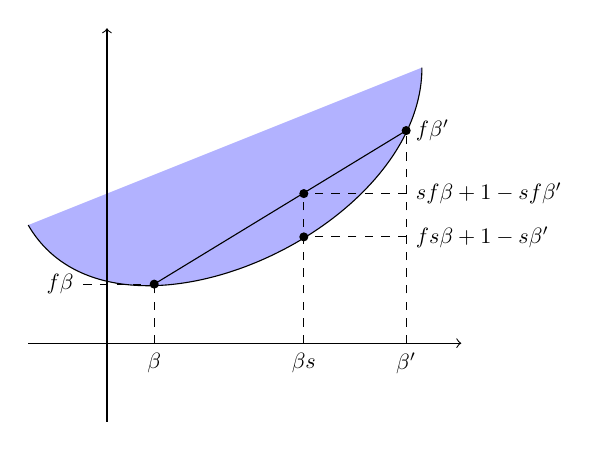
\begin{tikzpicture}
\draw (-1,1.5) to[out=300,in=270] (4,3.5)[fill= blue!30];
\draw [->] (-1,0) -- (4.5,0); % x-aksen
\draw[->] (0,-1) -- (0,4); % y-aksen
\draw (0.6,0.75) -- (3.80,2.7);
\draw [fill] (0.6,0.75) circle [radius=0.05];
\draw [fill] (3.80,2.7) circle [radius=0.05];
\draw [fill] (2.5,1.9) circle [radius=0.05];
\draw [fill] (2.5,1.35) circle [radius=0.05];
\draw [dashed] (-0.3,0.75) node [left] {\scalebox{0.8}{$f \del{\beta}$}} -- (0.6,0.75);
\draw [dashed] (0.6,0) node [below] {\scalebox{0.8}{$\beta$}} -- (0.6,0.75);
\draw [dashed] (2.5,0) node [below] {\scalebox{0.8}{$\beta \del{s}$}} -- (2.5,1.9);
\draw [dashed] (3.80,0) node [below] {\scalebox{0.8}{$\beta'$}} -- (3.80,2.7);

\draw [dashed] (3.80,2.7) node [right] {\scalebox{0.8}{$f \del{\beta'}$}} -- (3.80,2.7);
\draw [dashed] (3.80,1.9) node [right] {\scalebox{0.8}{$ sf \del{\beta} + \del{1-s} f \del{\beta'}$}} -- (2.5,1.9);
\draw [dashed] (3.80,1.35) node [right] {\scalebox{0.8}{$f \del{s \beta + \del{1-s} \beta'}$}} -- (2.5,1.35);
\end{tikzpicture}
}
\caption{For en konveks funktion ligger linjen \(s f \del{\beta} + \del{1-s} f \del{\beta'}\) altid over funktionsværdien \(f \del{s \beta + \del{1-s} \beta'}\).} \label{fig:konveks}
\end{figure}
%